% !TeX program = xelatex
% !TeX root = representation_final.tex
% !TeX encoding = UTF-8
% !TeX spellcheck = en_US
% arara: xelatex: { interaction: nonstopmode, synctex: yes }
% arara: xelatex: { interaction: nonstopmode, synctex: yes }
%
% Auto-build note:
% - VS Code LaTeX Workshop: enable "latex-workshop.latex.autoBuild.run": "onSave".
% - TeXstudio/TeXShop can use the magic comments above to choose XeLaTeX.
% - Manual command from final_submission/:
%   bash watch_representation_final.sh
% - Automatic watch (save-to-recompile):
%   bash watch_representation_final.sh representation_final.tex
%
% Merged: covariance_final.tex (Stabilizing & Accelerating Mahalanobis MMD) placed before
% the CNN Representation-Assisted MMMD content.

\documentclass[aspectratio=169,10pt]{beamer}

\usepackage{fontspec}
\usepackage{graphicx}
\usepackage{booktabs}
\usepackage{array}
\usepackage{tabularx}
\usepackage{amsmath,amssymb}
\usepackage{xcolor}
\usepackage{tikz}
\usetikzlibrary{arrows.meta,positioning,calc}

\graphicspath{{figures/}}

% Fudan-inspired, projector-safe palette.
\definecolor{fudanblue}{HTML}{0B4EA2}
\definecolor{fudanmid}{HTML}{2F68B2}
\definecolor{fudanlight}{HTML}{EEF4FC}
\definecolor{textgray}{HTML}{333333}
\definecolor{mutedgray}{HTML}{6B7280}
\definecolor{rulegray}{HTML}{D7DCE5}
\definecolor{accentorange}{HTML}{D97904}
\definecolor{accentgreen}{HTML}{008A5B}

\newcommand{\pos}[1]{\textcolor{fudanblue}{#1}}
\newcommand{\warn}[1]{\textcolor{accentorange}{#1}}
\newcommand{\HL}[1]{\textcolor{accentgreen}{#1}}

\setbeamertemplate{navigation symbols}{}
\setbeamersize{text margin left=0.72cm,text margin right=0.72cm}
\setbeamercolor{normal text}{fg=textgray,bg=white}
\setbeamercolor{frametitle}{fg=fudanblue,bg=white}
\setbeamercolor{item}{fg=fudanblue}
\setbeamercolor{caption name}{fg=fudanblue}
\setbeamerfont{frametitle}{series=\bfseries,size=\Large}
\setbeamerfont{framesubtitle}{size=\small}
\setbeamerfont{title}{series=\bfseries,size=\LARGE}
\setbeamerfont{subtitle}{size=\large}
\setbeamerfont{itemize/enumerate body}{size=\small}
\setbeamerfont{itemize/enumerate subbody}{size=\small}

\setbeamertemplate{itemize item}{\color{fudanblue}\scriptsize$\blacksquare$}
\setbeamertemplate{itemize subitem}{\color{fudanblue}\scriptsize$\blacktriangleright$}

% Titled rounded boxes used as "algorithm boxes" (from covariance_final.tex).
\setbeamertemplate{blocks}[rounded][shadow=false]
\setbeamercolor{block title}{fg=white,bg=fudanblue}
\setbeamercolor{block body}{fg=textgray,bg=fudanlight}

\newcommand{\maybelogo}[2]{%
  \IfFileExists{figures/#1}{\includegraphics[#2]{#1}}{}%
}

\newcommand{\fig}[2][]{%
  \IfFileExists{figures/#2}{\includegraphics[#1]{#2}}{%
    \fbox{\begin{minipage}[c][0.34\textheight][c]{0.94\linewidth}
      \centering\small Missing figure:\\ \texttt{\detokenize{figures/#2}}
    \end{minipage}}%
  }%
}

\newcommand{\keyline}[1]{%
  \vspace{0.04cm}
  \noindent\begin{tabular}{@{}m{2.2pt}@{\hspace{0.55em}}m{0.90\linewidth}@{}}
    {\color{accentgreen}\rule{2.2pt}{1.35em}} & \textbf{#1}
  \end{tabular}
  \vspace{0.09cm}
}

\newcommand{\metric}[2]{%
  \begin{minipage}[t]{0.30\linewidth}
    \centering
    {\Large\bfseries\color{fudanblue}#1}\\[-1pt]
    {\scriptsize\color{mutedgray}#2}
  \end{minipage}
}

\newcommand{\smallnote}[1]{%
  {\scriptsize\color{mutedgray}#1}
}

% --- math shorthands (source-level only; render exactly as in arXiv:2302.10687) ---
\newcommand{\sfK}{\mathsf{K}}                      % kernel, sans-serif as in paper
\newcommand{\Sig}{\hat{\boldsymbol{\Sigma}}}        % covariance estimate
\newcommand{\Kcg}{\hat{\mathbf{K}}^{\circ}}         % centered Gram matrix: (1/m) C_m K C_m
\newcommand{\mmdvec}{\mathrm{MMD}^2[\mathcal K,\mathcal X_m,\mathcal Y_n]} % MMD vector, full paper form
\newcommand{\rhohat}{\hat{\rho}}

\setbeamertemplate{frametitle}{%
  \begin{tikzpicture}[remember picture,overlay]
    \node[anchor=north west,inner sep=0pt] at ($(current page.north west)+(0.78cm,0cm)$)
      {\maybelogo{fudan_logo.png}{height=1.34cm}};
    \node[anchor=north west,align=left,text width=0.74\paperwidth] at ($(current page.north west)+(2.58cm,-0.47cm)$)
      {{\usebeamerfont{frametitle}\color{fudanblue}\insertframetitle\par}
       {\usebeamerfont{framesubtitle}\color{fudanblue!72!black}\insertframesubtitle\par}};
  \end{tikzpicture}
  \vspace{1.42cm}
}

\setbeamertemplate{footline}{%
  \leavevmode
  \hbox{\hspace{0.72cm}\scriptsize\color{mutedgray}\insertframenumber/\inserttotalframenumber}
  \vspace{0.20cm}
}


\begin{document}

% ===================================================================
% PART I: Covariance-Geometry — Stabilizing & Accelerating Mahalanobis MMD
% ===================================================================

\title{Stabilizing \& Accelerating Mahalanobis MMD}
\subtitle{Reboosting the power of two sample test}
\author{Ruijie Li, Ziheng Zheng, Dechao Huang, Yao yu}
\date{June 2026}

{% title page
\begin{frame}[plain]
  \begin{tikzpicture}[remember picture,overlay]
    \fill[white] (current page.south west) rectangle (current page.north east);
    \begin{scope}
      \clip ($(current page.south east)+(-5.85cm,0cm)$) --
            ($(current page.north east)+(-2.62cm,0cm)$) --
            (current page.north east) --
            (current page.south east) -- cycle;
      \IfFileExists{figures/fudan_background.png}{%
        \node[anchor=south east,inner sep=0pt] at (current page.south east)
          {
\includegraphics[width=0.68\paperwidth,height=\paperheight]{fudan_background.png}};
      }{%
        \fill[fudanblue] (current page.south west) rectangle (current page.north east);
      }
    \end{scope}
    \node[anchor=north west,inner sep=0pt] at ($(current page.north west)+(0.78cm,0cm)$)
      {\maybelogo{fudan_logo.png}{height=1.75cm}};
    \node[anchor=north west,inner sep=0pt] at ($(current page.north west)+(0.88cm,-2.58cm)$) {%
      \begin{minipage}{0.60\paperwidth}
        \raggedright
        {\color{textgray}\usebeamerfont{title}\inserttitle\par}
        \vspace{0.20cm}
        {\color{textgray}\usebeamerfont{subtitle}\insertsubtitle\par}
        \vspace{0.58cm}
        {\color{textgray}\large\insertauthor\par}
        \vspace{0.12cm}
        {\color{textgray}\insertdate\par}
      \end{minipage}
    };
  \end{tikzpicture}
\end{frame}
}

% ===================================================================
% SETUP -- what a two-sample test is
% ===================================================================
\begin{frame}{Two-Sample Testing}{The question, and what a test must provide}

\vspace{0.04cm}
We observe two samples and ask whether they come from the \emph{same} distribution:
\[
  \mathcal X_m=\{X_1,\dots,X_m\}\sim P,\qquad
  \mathcal Y_n=\{Y_1,\dots,Y_n\}\sim Q,
  \qquad
  H_0:\ P=Q \ \ \text{vs}\ \ H_1:\ P\ne Q.
\]

\vspace{0.30cm}
A test needs two ingredients:
\begin{itemize}
  \item a \textbf{statistic} that measures how different the two samples look;
  \item a \textbf{decision rule} -- reject $H_0$ when that statistic is large.
\end{itemize}

\vspace{0.30cm}
\keyline{The whole talk is about building a good statistic and keeping it reliable.}

\end{frame}

% ===================================================================
% MMD -- the single-kernel building block
% ===================================================================
\begin{frame}{Maximum Mean Discrepancy (MMD)}{The single-kernel building block}

\vspace{0.04cm}
MMD measures the distance between two distributions through a \textbf{kernel} $\sfK$
(a similarity function). Its key property: $\ \mathrm{MMD}=0 \iff P=Q$.

\vspace{0.25cm}
From data we estimate it by averaging \emph{within}-sample similarities minus
\emph{between}-sample similarities:
\[
  \mathrm{MMD}^2[\sfK,\mathcal X_m,\mathcal Y_n]
  = \underbrace{\mathcal W_{\mathcal X_m} + \mathcal W_{\mathcal Y_n}}_{\text{within}}
    \;-\; 2\,\underbrace{\mathcal B_{\mathcal X_m,\mathcal Y_n}}_{\text{between}} .
\]
The single-kernel test rejects $H_0$ when this estimate is large.

\vspace{0.25cm}
\keyline{Weakness: for a Gaussian kernel $\sfK_\sigma(x,y)=e^{-\|x-y\|^2/\sigma^2}$, the bandwidth $\sigma$ fixes the scale -- small $\sigma$ sees local, large $\sigma$ sees global differences. One $\sigma$ is a gamble.}

\end{frame}

% ===================================================================
% MMMD -- aggregate + statistic + rule
% ===================================================================
\begin{frame}{The Paper's Method: Mahalanobis MMD}{Combine many bandwidths into one statistic}

\vspace{0.04cm}
Instead of betting on one bandwidth, use $r$ kernels $\sfK_1,\dots,\sfK_r$ and collect their
MMD estimates into a vector $\mmdvec$. Simply summing them would \emph{double-count}
correlated kernels, so we combine them by their Mahalanobis distance -- weighting by the
inverse covariance $\Sig^{-1}$:
\[
  \boxed{\;T_{m,n}=\big(\mmdvec\big)^{\!\top}\,\Sig^{-1}\,\big(\mmdvec\big)\;}
\]

\vspace{0.20cm}
\textbf{Decision rule.} Reject $H_0$ when $T_{m,n}$ exceeds a cut-off; the cut-off is
calibrated by a multiplier bootstrap. A large
$T_{m,n}$ means the kernels \emph{jointly} detect a difference.

\end{frame}
% ===================================================================
% PART II: CNN Representation-Assisted MMMD
% ===================================================================

\title{CNN Representation-Assisted MMMD}
\subtitle{From Power Improvement to Biomedical Domain-Shift Interpretation}
\author{Individual Component}
\date{June 2026}

{% title page
\begin{frame}[plain]
  \begin{tikzpicture}[remember picture,overlay]
    \fill[white] (current page.south west) rectangle (current page.north east);
    \begin{scope}
      \clip ($(current page.south east)+(-5.85cm,0cm)$) --
            ($(current page.north east)+(-2.62cm,0cm)$) --
            (current page.north east) --
            (current page.south east) -- cycle;
      \IfFileExists{figures/fudan_background.png}{%
        \node[anchor=south east,inner sep=0pt] at (current page.south east)
          {
\includegraphics[width=0.68\paperwidth,height=\paperheight]{fudan_background.png}};
      }{%
        \fill[fudanblue] (current page.south west) rectangle (current page.north east);
      }
    \end{scope}
    \node[anchor=north west,inner sep=0pt] at ($(current page.north west)+(0.78cm,0cm)$)
      {\maybelogo{fudan_logo.png}{height=1.75cm}};
    \node[anchor=north west,inner sep=0pt] at ($(current page.north west)+(0.88cm,-2.58cm)$) {%
      \begin{minipage}{0.60\paperwidth}
        \raggedright
        {\color{textgray}\usebeamerfont{title}\inserttitle\par}
        \vspace{0.20cm}
        {\color{textgray}\usebeamerfont{subtitle}\insertsubtitle\par}
        \vspace{0.58cm}
        {\color{textgray}\large\insertauthor\par}
        \vspace{0.12cm}
        {\color{textgray}\insertdate\par}
      \end{minipage}
    };
  \end{tikzpicture}
\end{frame}
}

% ===================================================================
% Part 0: MMMD Kernel Extensions — Numerical Experiments (Andrew Zheng)
% ===================================================================

\begin{frame}{MMMD Framework}{Mahalanobis Multi-Kernel Maximum Mean Discrepancy}
\keyline{A multi-kernel two-sample test with decorrelated kernel aggregation and multiplier bootstrap.}
\vspace{0.15cm}
\begin{center}
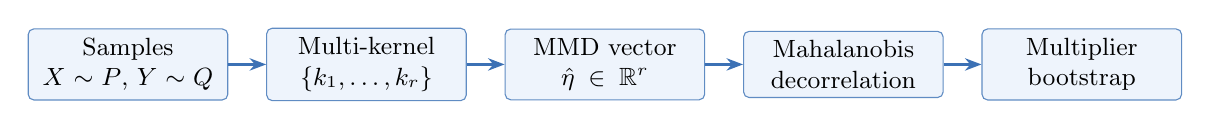
\begin{tikzpicture}[
  node distance=0.48cm,
  flowbox/.style={draw=fudanblue!65, fill=fudanlight, rounded corners=2pt,
                  minimum height=0.82cm, text width=2.30cm, align=center, font=\small},
  arr/.style={-{Stealth[length=2.1mm]}, thick, draw=fudanblue!80}
]
  \node[flowbox] (xy) {Samples\\$X \sim P$, $Y \sim Q$};
  \node[flowbox, right=of xy] (kern) {Multi-kernel\\$\{k_1,\ldots,k_r\}$};
  \node[flowbox, right=of kern] (vec) {MMD vector\\$\hat{\eta} \in \mathbb{R}^r$};
  \node[flowbox, right=of vec] (decor) {Mahalanobis\\decorrelation};
  \node[flowbox, right=of decor] (boot) {Multiplier\\bootstrap};
  \draw[arr] (xy) -- (kern);
  \draw[arr] (kern) -- (vec);
  \draw[arr] (vec) -- (decor);
  \draw[arr] (decor) -- (boot);
\end{tikzpicture}
\end{center}
\vspace{0.12cm}
\begin{columns}[T,totalwidth=\linewidth]
\begin{column}{0.32\linewidth}
\textbf{\pos{Kernel families}}
\begin{itemize}
  \item GEXP: RBF exponential bandwidth grid
  \item LAP: Laplace kernel family
  \item MIXED: combined RBF + Laplace
\end{itemize}
\end{column}
\begin{column}{0.32\linewidth}
\textbf{Key components}
\begin{itemize}
  \item $\hat{\Sigma}$: kernel covariance estimation
  \item Ridge stabilization: $\lambda = 10^{-5} \cdot \min(\mathrm{diag}(\hat{\Sigma}))$
  \item Vectorised bootstrap for $\alpha$-grid scan
\end{itemize}
\end{column}
\begin{column}{0.32\linewidth}
\textbf{\HL{Extensions}}
\begin{itemize}
  \item Graph-MMMD: kNN graph + heat kernel
  \item Skew-normal, MV-Laplace, Normal-t mixture
  \item Parallel computing backend
\end{itemize}
\end{column}
\end{columns}
\end{frame}
% ===================================================================
% Covariance -- the engine
% ===================================================================
\begin{frame}{The Covariance $\Sig$}{The engine behind the Mahalanobis weighting}

\vspace{0.04cm}
The weighting needs $\Sig$: the covariance of the $r$ MMD estimates under $H_0$. It is
what puts correlated kernels on a common footing. Its empirical estimate (paper, Eq.~15) is
\[
  \hat\sigma_{ab}
  =\frac{2}{\rhohat^{2}(1-\rhohat)^{2}}\cdot\frac{1}{m^{2}}
   \sum_{1\le i,j\le m}\hat{\sfK}^{\circ}_a(X_i,X_j)\,\hat{\sfK}^{\circ}_b(X_i,X_j),
  \qquad \rhohat=\tfrac{m}{m+n}.
\]

\vspace{0.20cm}
Every entry is built from \textbf{kernel Gram matrices} on the $X$ sample -- and that is
exactly where both of my fixes act.

\end{frame}

% ===================================================================
% Gram + geometry -> ill-conditioned + expensive
% ===================================================================
\begin{frame}{Gram Matrices and a Hidden Geometry}{Why $\Sig$ is fragile and costly}

\vspace{0.04cm}
The \textbf{Gram matrix} of a kernel collects all pairwise similarities,
$\hat{\sfK}_a=\{\sfK_a(X_i,X_j)\}$. After centering, $\Sig$ turns out to be a
``Gram matrix of Gram matrices'' -- each entry is an inner product of two centered
Gram matrices:
\[
  \hat\sigma_{ab}\ \propto\ \big\langle \Kcg_a,\,\Kcg_b\big\rangle_F,
  \qquad \Kcg_a=\tfrac1m C_m\hat{\sfK}_aC_m
  \qquad\Longrightarrow\qquad
  \Sig=\text{Gram matrix of }\{\operatorname{vec}(\Kcg_a)\}.
\]

\vspace{0.18cm}
\begin{columns}[T,totalwidth=\linewidth]
\begin{column}{0.50\linewidth}
\textbf{\warn{Ill-conditioned.}} Redundant bandwidths give near-identical Gram matrices,
so $\Sig$ is near-singular; then $\Sig^{-1}$ blows up estimation noise and $H_0$ is
over-rejected.
\end{column}
\begin{column}{0.46\linewidth}
\textbf{\warn{Expensive.}} A naive build needs $R^2$ such inner products.
\end{column}
\end{columns}

\end{frame}

% ===================================================================
% My extension overview
% ===================================================================
\begin{frame}{My Extension: Two Construction-Layer Fixes}{Attack the cause, not the symptom}

\vspace{0.18cm}
\begin{itemize}\setlength\itemsep{0.45cm}
  \item \textbf{\pos{Stability.}} $\Sig$ is ill-conditioned. \HL{Fix:} prune the redundant
        kernels \emph{before} inverting -- lazy pivoted Cholesky.
  \item \textbf{\pos{Speed.}} The naive $O(R^2)$ build is slow. \HL{Fix:} exploit the
        Gaussian/Laplace product structure -- multiplicative closure.
\end{itemize}

\vspace{0.35cm}
Both act while $\Sig$ is being \emph{built}. The paper's only safeguard is a fixed ridge
$(\Sig+\lambda I)^{-1}$ added at the \emph{solve} step, which masks the problem rather than
removing it.

\end{frame}

% ===================================================================
% Fix 1 -- stability
% ===================================================================
\begin{frame}{Fix 1 -- Stability: Lazy Pivoted Cholesky}{Keep only kernels that add something new}

\vspace{0.04cm}
\textbf{Idea.} Go greedily: each round keep the kernel whose Gram matrix is
\emph{least explained} by the ones already chosen, and stop once the rest add almost
nothing. Redundant kernels are dropped, so $R\to q\ll R$ and $\Sig$ is well-conditioned again.
``\emph{Lazy}'': a covariance column is computed only when its kernel is picked, so the full
$R\times R$ matrix is never formed.

\vspace{0.12cm}
\begin{block}{Lazy Pivoted-Cholesky Kernel Selection}
\small
\begin{enumerate}\setlength\itemsep{2.2pt}
  \item residuals $r_j \leftarrow \Sig_{jj}$;\quad pivot $p_t=\arg\max_j r_j$;\quad
        \textbf{stop} if $r_{p_t}\le \varepsilon\max_j \Sig_{jj}$.
  \item fetch column $\mathcal C(p_t)=\Sig_{\cdot,p_t}$ (lazy);\quad
        $L_{j,t}=\big(\mathcal C(p_t)_j-\textstyle\sum_{s<t}L_{j,s}L_{p_t,s}\big)/\sqrt{r_{p_t}}$.
  \item update residuals $r_j \leftarrow r_j-L_{j,t}^{2}$;\quad repeat.
\end{enumerate}
\end{block}

\end{frame}

% ===================================================================
% Fix 2 -- speed
% ===================================================================
\begin{frame}{Fix 2 -- Speed: Multiplicative Closure}{Reuse one shared function instead of $R^2$ scans}

\vspace{0.04cm}
\textbf{Idea.} Gaussian/Laplace kernels multiply into another kernel of the same
family. So a covariance entry depends only on the \emph{sum} of the two bandwidth parameters,
through a single shared function $H$:
\[
  \sfK_{t_a}\sfK_{t_b}=\sfK_{t_a+t_b}\ \ (t=1/\sigma^2),
  \qquad
  H(u)=\sum_{i,j} e^{-u D_{ij}},\quad D_{ij}=\|X_i-X_j\|^2 .
\]
On an arithmetic grid, $t_a+t_b$ takes only $2R-1$ distinct values, so we compute $O(R)$
values of $H$ rather than $R^2$.

\vspace{0.22cm}
\begin{center}
Covariance cost:\quad
$\underbrace{O(R^2 m^3 + B R m^2)}_{\text{naive}}
\;\longrightarrow\;
\underbrace{O(R m^2 + B q m^2)}_{\text{closure + selection}}$
\end{center}

\vspace{0.10cm}
\keyline{The heavy $m^2$ work is cached once; later steps (and each lazy column query) are cheap.}

\end{frame}

% ===================================================================
% EXPERIMENTS -- one figure per page
% ===================================================================
\begin{frame}{Experiments: Power}{Synthetic Gaussian scale shift -- matches the paper}

\begin{columns}[c,totalwidth=\linewidth]
\begin{column}{0.60\linewidth}
  \centering
  \fig[width=\linewidth,height=0.66\textheight,keepaspectratio]{Figure1b_with_NewMethod.pdf}
\end{column}
\begin{column}{0.37\linewidth}
  $d=2$ variance shift;\\ $x$-axis: sample size $n$,\\ $y$-axis: power.

  \vspace{0.45cm}
  The new method tracks the paper's multi-kernel test to within $4$ pp, and both
  clearly beat the single-kernel test.
\end{column}
\end{columns}

\end{frame}

\begin{frame}{Experiments: Speed}{Large speed-up at equal kernel count}

\begin{columns}[c,totalwidth=\linewidth]
\begin{column}{0.60\linewidth}
  \centering
  \fig[width=\linewidth,height=0.66\textheight,keepaspectratio]{TimeComparison_total.pdf}
\end{column}
\begin{column}{0.37\linewidth}
  $d=5$;\\ $x$-axis: sample size $n$,\\ $y$-axis: time per iteration.

  \vspace{0.45cm}
  At the same $R=13$: covariance $\sim16\times$ and end-to-end $\sim4.8\times$ faster;
  cost grows \emph{linearly} in $R$, not quadratically.
\end{column}
\end{columns}

\end{frame}

% -------------------------------------------------------------------
\begin{frame}{Task 1: $\varepsilon$-Contamination Sensitivity}{How much $t_{10}$ contamination can MMMD detect?}
\begin{columns}[T,totalwidth=\linewidth]
\begin{column}{0.55\linewidth}
  \centering
  \fig[width=\linewidth]{mmmd_epsilon_sensitivity.png}
\end{column}
\begin{column}{0.40\linewidth}
  \vspace{0.3cm}
  {\large\bfseries Setup}\\[0.2em]
  $P = \mathcal{N}(0,\Sigma)$, \quad $Q = (1-\varepsilon)\mathcal{N}(0,\Sigma) + \varepsilon \cdot t_{10}(0,\Sigma)$
  \vspace{0.3cm}

  \begin{itemize}
    \item $d=30$, $n=100$, $\rho=0.5$ (AR(1))
    \item GEXP kernel, $r=5$, $B=500$, $N=150$
  \end{itemize}
  \vspace{0.3cm}

  \keyline{$\varepsilon_{\min} = 0.625$}
  \vspace{0.1cm}
  {\small Power reaches 0.80 when 62.5\% of $Q$ is $t_{10}$.\\
  Steep transition: $\varepsilon \in [0.45, 0.65]$, power rises $0.57 \to 0.80$.}
\end{column}
\end{columns}
\end{frame}

% -------------------------------------------------------------------
\begin{frame}{Task 2: Variance-Scale $k$ Sensitivity}{How small a variance change can MMMD detect?}
\begin{columns}[T,totalwidth=\linewidth]
\begin{column}{0.48\linewidth}
  \centering
  \fig[width=\linewidth]{mmmd_variance_sensitivity.png}
\end{column}
\begin{column}{0.48\linewidth}
  \vspace{0.2cm}
  {\large\bfseries Setup}\\[0.15em]
  $P = \mathcal{N}(0,\Sigma_0)$, \quad $Q = \mathcal{N}(0, k \cdot \Sigma_0)$
  \vspace{0.2cm}

  \begin{center}
  \small
  \begin{tabular}{lcc}
  \toprule
  Method & $k_{\min}$ & Power at $k=1.20$ \\
  \midrule
  \textbf{Mixed MMMD} & \textbf{1.25} & 0.71 \\
  Gauss MMMD & 1.25 & 0.79 \\
  LAP MMMD & 1.25 & 0.75 \\
  Gauss MMD (single) & \warn{1.40} & \warn{0.18} \\
  \bottomrule
  \end{tabular}
  \end{center}
  \vspace{0.10cm}

  \keyline{MMMD: 15\% earlier detection than single-kernel MMD}
  \vspace{0.05cm}
  {\footnotesize At $k=1.20$, MMMD achieves 71--79\% power while\\
  single-kernel MMD stays at 18\% — a 4$\times$ gap.}
\end{column}
\end{columns}
\end{frame}

% -------------------------------------------------------------------
\begin{frame}{Task 3a: Type-I Error Calibration}{Does MMMD maintain nominal level under the null?}
\vspace{0.12cm}
\begin{columns}[T,totalwidth=\linewidth]
\begin{column}{0.48\linewidth}
  \centering
  {\large\bfseries Type-I Error @ $\alpha=0.05$}\\[0.25em]
  \begin{tabular}{lccc}
  \toprule
  Family & $r=3$ & $r=5$ & $r=10$ \\
  \midrule
  GEXP & 0.020 & 0.055 & \warn{0.120} \\
  LAP  & 0.045 & 0.045 & 0.050 \\
  MIXED& 0.050 & 0.050 & 0.070 \\
  \bottomrule
  \end{tabular}
  \vspace{0.2cm}

  \begin{itemize}
    \item $r=3,5$: well-calibrated within $[0.02, 0.055]$
    \item $r=10$ GEXP: inflation to 0.12 — too many kernels degrade $\hat{\Sigma}$ estimation
    \item LAP maintains calibration at all $r$ levels
  \end{itemize}
\end{column}
\begin{column}{0.48\linewidth}
  \centering
  \fig[width=\linewidth]{mmmd_roc_curves.png}
\end{column}
\end{columns}
\vspace{-0.1cm}
\begin{center}
\smallnote{$d=30$, $n=100$, $B=500$, $N=200$ trials per cell.  Warning system flags Type-I outside $[0.02, 0.08]$.}
\end{center}
\end{frame}

% -------------------------------------------------------------------
\begin{frame}{Task 3b: ROC Analysis}{Power–Type-I trade-off across kernel families}
\begin{columns}[T,totalwidth=\linewidth]
\begin{column}{0.52\linewidth}
  \fig[width=\linewidth]{mmmd_roc_curves.png}
\end{column}
\begin{column}{0.44\linewidth}
  \vspace{0.3cm}
  {\large\bfseries Vectorised ROC scan}\\[0.2em]
  \begin{itemize}
    \item Single bootstrap run → all $\alpha$ thresholds
    \item $H_1$: variance scale $k=1.15$
    \item $\alpha \in [0, 1]$, step $0.01$
  \end{itemize}
  \vspace{0.4cm}

  \begin{center}
  \begin{tabular}{lccc}
  \toprule
  Family & FPR & TPR @ $\alpha=0.05$ \\
  \midrule
  GEXP  & 0.045 & 0.500 \\
  LAP   & 0.045 & 0.495 \\
  MIXED & 0.050 & 0.435 \\
  \bottomrule
  \end{tabular}
  \end{center}
  \vspace{0.15cm}
  {\small All families: FPR close to nominal 0.05;\\
  ROC curves well above diagonal → valid test.}
\end{column}
\end{columns}
\end{frame}

% -------------------------------------------------------------------
\begin{frame}{Task 4a: Graph-MMMD Extension}{kNN graph kernel with heat/diffusion kernel}
\keyline{Graph-MMMD: build kNN graph → graph Laplacian → heat kernel $K_t = \exp(-tL)$ → MMMD pipeline.}
\vspace{0.10cm}
\begin{columns}[T,totalwidth=\linewidth]
\begin{column}{0.50\linewidth}
  \centering
  \fig[width=\linewidth]{mmmd_graph_type1.png}
\end{column}
\begin{column}{0.46\linewidth}
  \vspace{0.15cm}
  {\large\bfseries Type-I under 4 null distributions}\\[0.18em]
  \begin{tabular}{lc}
  \toprule
  Null Distribution & Type-I Error \\
  \midrule
  AR(1) Normal ($\rho=0.5$) & 0.027 \\
  AR(1) Normal, $k=1.5$ & 0.020 \\
  Skew-Normal ($\alpha=5$) & 0.020 \\
  Multivariate Laplace & 0.033 \\
  \bottomrule
  \end{tabular}
  \vspace{0.25cm}
  \begin{itemize}
    \item All $\leq 0.053$ — well-calibrated across distributions
    \item Non-Gaussian and asymmetric nulls do not inflate Type-I
  \end{itemize}
\end{column}
\end{columns}
\end{frame}

% -------------------------------------------------------------------
\begin{frame}{Task 4b: Skewness Robustness}{Graph-MMMD calibration across skewness levels}
\begin{columns}[T,totalwidth=\linewidth]
\begin{column}{0.46\linewidth}
  \centering
  \fig[width=\linewidth]{mmmd_skew_type1.png}
\end{column}
\begin{column}{0.50\linewidth}
  \vspace{0.2cm}
  {\large\bfseries Skewness sweep}\\[0.15em]
  {\footnotesize Skew-Normal with shape $\alpha$ mapped to standardized skewness.}\\[0.2em]

  \small
  \begin{tabular}{lcc}
  \toprule
  Std.\ Skewness & Shape $\alpha$ & Type-I \\
  \midrule
  0.00 & 0.00 & 0.020 \\
  0.10 & 0.87 & 0.020 \\
  0.25 & 1.35 & 0.047 \\
  0.50 & 2.17 & 0.033 \\
  0.75 & 3.64 & 0.053 \\
  0.90 & 6.30 & 0.020 \\
  \bottomrule
  \end{tabular}
  \vspace{0.15cm}

  \keyline{Type-I $\leq 0.053$ even at extreme skewness (0.90)}
  \vspace{0.05cm}
  {\footnotesize $\alpha$ found via \texttt{uniroot()} from stochastic representation,\\
  no external dependencies.}
\end{column}
\end{columns}
\end{frame}

% -------------------------------------------------------------------
\begin{frame}{Fig.2 Reproduction: Mixture Distribution Power}{MMMD vs single-kernel MMD under normal-$t$ mixture}
\begin{columns}[T,totalwidth=\linewidth]
\begin{column}{0.46\linewidth}
  \centering
  \fig[width=\linewidth]{mmmd_fig2_mixture.png}
\end{column}
\begin{column}{0.54\linewidth}
  \vspace{0.04cm}
  {\large\bfseries Setup}\\[0.06em]
  \scriptsize
  $\begin{aligned}
  P &= (1-p)\mathcal{N}(0,\Sigma_0) + p \cdot t_{\nu}(0,\Sigma_0)\\
  Q &= (1-p)\mathcal{N}(0,\Sigma_1) + p \cdot t_{\nu}(0,\Sigma_1)
  \end{aligned}$
  \vspace{0.06cm}

  {\scriptsize $\Sigma_1 = 1.25 \cdot \Sigma_0$, $d=30$, $\rho=0.5$, $\nu=10$}\\[0.08em]

  \begin{center}
  \resizebox{\linewidth}{!}{%
  \begin{tabular}{lcccc}
  \toprule
  $p$ & MMMD-Mix & MMMD-Gauss & MMMD-LAP & MMD-Gauss \\
  \midrule
  0.0 & \textbf{0.96} & 0.89 & 0.94 & 0.46 \\
  0.4 & 0.80 & 0.84 & 0.71 & 0.31 \\
  1.0 & 0.58 & 0.69 & 0.53 & 0.35 \\
  \bottomrule
  \end{tabular}%
  }
  \end{center}
  \vspace{0.06cm}

  {\scriptsize\keyline{MMMD methods: 2--5$\times$ the power of single-kernel baselines}}
  {\scriptsize MMMD advantage persists across all mixture proportions $p$.}
\end{column}
\end{columns}
\end{frame}

% -------------------------------------------------------------------
\begin{frame}{Numerical Extensions — Summary}{Key findings from the MMMD kernel framework}
\vspace{0.08cm}
\begin{tabularx}{0.96\linewidth}{>{\bfseries\color{fudanblue}}p{0.26\linewidth}X}
\toprule
Extension & Main Finding \\
\midrule
$\varepsilon$-sensitivity
& MMMD detects contamination at $\varepsilon_{\min}=0.625$; power rises sharply in $[0.45,0.65]$. \\
\addlinespace[0.18em]
Variance $k$-sensitivity
& MMMD detects $k_{\min}=1.25$ vs.\ Gauss MMD $k_{\min}=1.40$; 15\% earlier, 4$\times$ gap at $k=1.20$. \\
\addlinespace[0.18em]
Type-I \& ROC
& Well-calibrated at $r=3,5$; $r=10$ GEXP inflates (0.12); LAP robust at all $r$. ROC confirms test validity. \\
\addlinespace[0.18em]
Graph-MMMD
& Type-I $\leq 0.053$ across 4 null distributions and 6 skewness levels (up to std.\ skewness 0.90). \\
\addlinespace[0.18em]
Fig.2 Mixture
& MMMD 2--5$\times$ single-kernel power across all $p$; Mixed MMMD best at $p=0$ (0.96 vs.\ 0.46). \\
\bottomrule
\end{tabularx}

\vspace{0.20cm}
\begin{center}
\smallnote{All experiments: $d=30$, AR(1) $\rho=0.5$, $B=500$, $N_{\text{trials}}=150$--$200$. Modular R/ library with parallel backend.}
\end{center}
\end{frame}

% -------------------------------------------------------------------
\begin{frame}{MNIST Reproduction}{Original-paper benchmark check}
\begin{columns}[T,totalwidth=\linewidth]
\begin{column}{0.49\linewidth}
  \centering
  {\large\bfseries Power}\\[0.25em]
  \fig[width=\linewidth]{mnist_cnn_power.png}
\end{column}
\begin{column}{0.49\linewidth}
  \centering
  {\large\bfseries Type-I error}\\[0.25em]
  \fig[width=\linewidth]{mnist_cnn_type1_error_two_nulls.png}
\end{column}
\end{columns}
\vspace{-0.05cm}
\begin{center}
\smallnote{Reproduction anchor: MNIST additive-noise power plus matched-null calibration.}
\end{center}
\end{frame}

% -------------------------------------------------------------------
\begin{frame}{Representation Choice}{Raw pixels versus CNN embeddings for image two-sample testing}
\begin{columns}[T,totalwidth=\linewidth]

\begin{column}{0.60\linewidth}
  \vspace{-0.15cm}
  \fig[width=\linewidth]{mnist_cnn_power.png}
\end{column}

\begin{column}{0.36\linewidth}

  \vspace{0.5em}
  \small
  \begin{itemize}
    \item Original MMMD improves kernel and bandwidth choice for a fixed input space.
    \item I compare raw pixels with CNN embeddings.
    \item Train CNN once, freeze it, cache embeddings, and run MMMD repeatedly.
    \item Multilayer variants: 3 components with one Gaussian per layer, or 15 components with five bandwidths per layer.
  \end{itemize}

\end{column}

\end{columns}
\end{frame}

% -------------------------------------------------------------------
\begin{frame}{CNN-MMMD}{A lightweight representation-assisted pipeline}
\keyline{Use MMMD on learned image features, not only on flattened pixels.}
\vspace{0.12cm}
\begin{center}
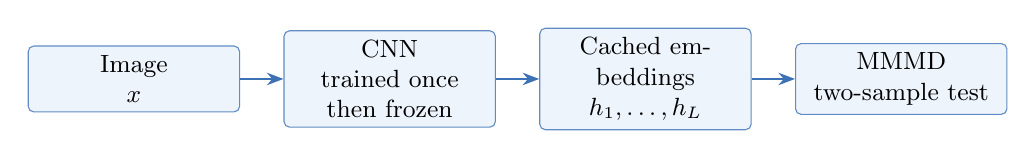
\begin{tikzpicture}[
  node distance=0.55cm,
  flowbox/.style={draw=fudanblue!65, fill=fudanlight, rounded corners=2pt,
                  minimum height=0.82cm, text width=2.45cm, align=center, font=\small},
  arr/.style={-{Stealth[length=2.1mm]}, thick, draw=fudanblue!80},
  note/.style={font=\scriptsize, color=mutedgray, align=center}
]
  \node[flowbox] (x) {Image\\$x$};
  \node[flowbox, right=of x] (cnn) {CNN trained once\\then frozen};
  \node[flowbox, right=of cnn] (emb) {Cached embeddings\\$h_1,\ldots,h_L$};
  \node[flowbox, right=of emb] (mmmd) {MMMD\\two-sample test};
  \draw[arr] (x) -- (cnn);
  \draw[arr] (cnn) -- (emb);
  \draw[arr] (emb) -- (mmmd);
\end{tikzpicture}
\end{center}
\vspace{0.08cm}
\begin{columns}[T,totalwidth=\linewidth]
\begin{column}{0.48\linewidth}
\textbf{\pos{Penultimate FC-128 embedding}}
\begin{itemize}
  \item compact, classifier-proximal representation
  \item enriched for tissue-discriminative information
\end{itemize}
\end{column}
\begin{column}{0.48\linewidth}
\textbf{\HL{Multilayer embedding}}
\begin{itemize}
  \item combines shallow, middle, and penultimate features
  \item keeps complementary low- and high-level cues
  \item extends MMMD from multi-kernel to multi-representation aggregation
\end{itemize}
\end{column}
\end{columns}
\end{frame}

% -------------------------------------------------------------------
\begin{frame}{Study Roadmap}{From representation testing to biomedical interpretation}

\vspace{0.7cm}

\begin{center}
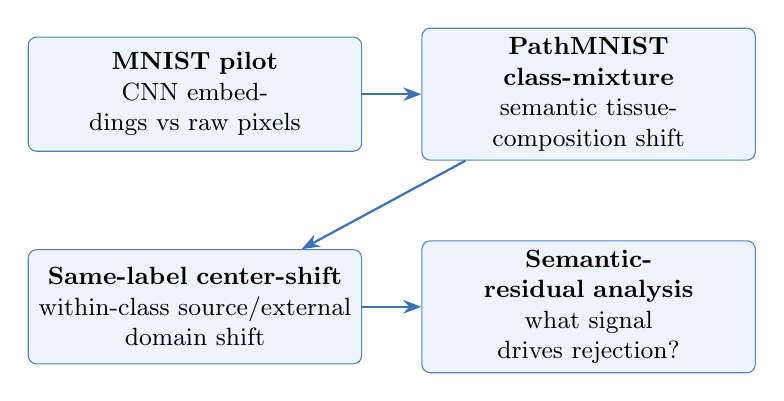
\begin{tikzpicture}[
  box/.style={
    draw=fudanblue!70,
    fill=fudanlight,
    rounded corners=3pt,
    text width=4.0cm,
    minimum height=1.45cm,
    align=center,
    font=\small
  },
  arr/.style={-{Stealth[length=2.3mm]}, thick, draw=fudanblue!80}
]

\node[box] (a) at (0, 3.7) {
  \textbf{MNIST pilot}\\
  CNN embeddings vs raw pixels
};

\node[box] (b) at (5.0, 3.7) {
  \textbf{PathMNIST class-mixture}\\
  semantic tissue-composition shift
};

\node[box] (c) at (0, 1) {
  \textbf{Same-label center-shift}\\
  within-class source/external domain shift
};

\node[box] (d) at (5.0, 1) {
  \textbf{Semantic-residual analysis}\\
  what signal drives rejection?
};

\draw[arr] (a) -- (b);
\draw[arr] (b) -- (c);
\draw[arr] (c) -- (d);

\end{tikzpicture}
\end{center}

\end{frame}

% -------------------------------------------------------------------
\begin{frame}{PathMNIST Class-Mixture}{Semantic tissue-composition shift}
\begin{columns}[T,totalwidth=\linewidth]
\begin{column}{0.57\linewidth}
  \fig[width=1.03\linewidth]{pathmnist_class_mixture_power.png}
\end{column}
\begin{column}{0.38\linewidth}
  {\large\bfseries Task}\\[0.25em]
  \texttt{mix635} vs \texttt{mix835}: two shared tissue components, one component changed.

  \vspace{0.65em}
  {\large\bfseries Result}\\[0.25em]
  CNN final and multilayer embeddings improve power over raw pixels.

  \vspace{0.45em}
  \small
  \begin{center}
  \begin{tabular}{lrr}
  \toprule
  Method & $n=90$ & $n=120$ \\
  \midrule
  Raw pixel & 0.497 & 0.636 \\
  FC-128 & 0.774 & \textbf{0.963} \\
  Multilayer G15 & \textbf{0.796} & 0.959 \\
  \bottomrule
  \end{tabular}
  \end{center}
\end{column}
\end{columns}
\end{frame}

% -------------------------------------------------------------------
\begin{frame}{Class-Mixture Type-I Check}{Matched null: \texttt{mix635} vs \texttt{mix635}}
\keyline{Matched-null rejection stays below $\alpha=0.05$.}
\vspace{-0.16cm}
\begin{center}
  \fig[width=0.78\linewidth]{pathmnist_class_type1_zoom.png}
\end{center}
\end{frame}

% -------------------------------------------------------------------
\begin{frame}{Same-Label Center Shift}{A biomedical domain-shift test}
\begin{center}
  \fig[width=0.90\linewidth]{pathmnist_center_shift_examples.png}
\end{center}
\vspace{-0.20cm}
\begin{columns}[T,totalwidth=0.92\linewidth]
\begin{column}{0.46\linewidth}
  \centering\small\textbf{\pos{Source / internal}}: official train holdout.
\end{column}
\begin{column}{0.46\linewidth}
  \centering\small\textbf{\warn{External}}: official external test center.
\end{column}
\end{columns}
\end{frame}

% -------------------------------------------------------------------
\begin{frame}{Center-Shift Result}{Same-label shift is strong, but representation profiles differ}

\vspace{-0.15cm}

\begin{center}
  \fig[width=0.78\linewidth]{pathmnist_center_shift_power.png}
\end{center}

\vspace{-0.10cm}

\begin{center}
\begin{minipage}[t]{0.36\linewidth}
\centering
{\normalsize\bfseries Rejection rate at $n=50$}\\[0.15em]
\scriptsize
\begin{tabular}{@{}lrr@{}}
\toprule
Method & Label 6 & Label 8 \\
\midrule
Raw pixel & 0.782 & 0.960 \\
FC-128 & 0.763 & 0.957 \\
Multilayer G15 & 0.989 & 0.975 \\
Multilayer single & \textbf{0.991} & \textbf{0.985} \\
\bottomrule
\end{tabular}
\end{minipage}
\hspace{0.035\linewidth}
\begin{minipage}[t]{0.43\linewidth}
\vspace{0.05cm}
\begin{itemize}
  \item Label 6: multilayer is much stronger than raw / FC-128.
  \item Label 8: raw pixel and FC-128 are already strong.
  \item Representation profile differs by label; next we try to locate the signal.
\end{itemize}
\end{minipage}
\end{center}

\end{frame}

% -------------------------------------------------------------------
\begin{frame}{Semantic vs Residual Signal}{What part of FC-128 drives rejection?}

\vspace{0.02cm}

{\normalsize
In a same-label test, MMMD rejection may come from different directions of the CNN representation.
}

\vspace{-0.12cm}

\begin{center}
\normalsize
\[
\text{logits}=Wh+b,\qquad
W_c=\left(I-\frac{1}{C}\mathbf{1}\mathbf{1}^{T}\right)W,\qquad
h=h_{\mathrm{sem}}+h_{\mathrm{res}}.
\]
\end{center}

\vspace{0.28cm}

\begin{columns}[T,totalwidth=0.94\linewidth]

\begin{column}{0.46\linewidth}
\centering
{\large\bfseries Classifier-used part}\\[0.38em]
{\large $h_{\mathrm{sem}}=P_{\mathrm{row}(W_c)}h$}\\[0.22em]
\begin{minipage}{0.88\linewidth}
\begin{itemize}
  \item affects class-relative logits
  \item aligned with tissue-discriminative directions
\end{itemize}
\end{minipage}
\end{column}

\begin{column}{0.46\linewidth}
\centering
{\large\bfseries Classifier-ignored part}\\[0.38em]
{\large $h_{\mathrm{res}}=h-h_{\mathrm{sem}}$}\\[0.22em]
\begin{minipage}{0.88\linewidth}
\begin{itemize}
  \item invisible to the linear classifier head
  \item may still contain domain or stain signal
\end{itemize}
\end{minipage}
\end{column}

\end{columns}

\vspace{0.30cm}

\begin{center}
{\scriptsize Diagnostic decomposition: used to interpret the rejection source, not to claim FC-128 is always strongest.}
\end{center}

\end{frame}

% -------------------------------------------------------------------
\begin{frame}{Semantic--Residual Result}{Task $\times$ component readout}
\keyline{Class-mixture is semantic/logit-aligned; label-8 center shift is residual-dominated.}
\vspace{0.10cm}
\begin{center}
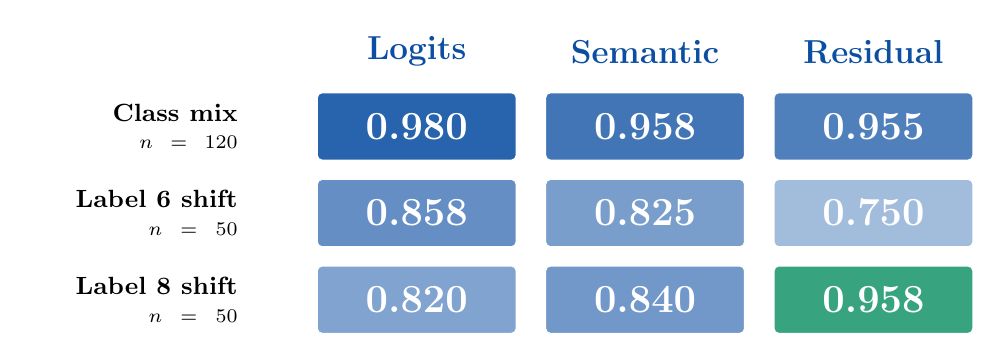
\begin{tikzpicture}[
  cell/.style={draw=white,line width=1.1pt,rounded corners=2pt,
               minimum width=2.55cm,minimum height=0.88cm,
               align=center,font=\Large\bfseries},
  rowlab/.style={anchor=east,text width=2.55cm,align=right,font=\small\bfseries},
  head/.style={font=\large\bfseries\color{fudanblue}}
]
  \node[head] at (2.05,3.05) {Logits};
  \node[head] at (4.95,3.05) {Semantic};
  \node[head] at (7.85,3.05) {Residual};

  \node[rowlab] at (-0.10,2.10) {Class mix\\[-1pt]\scriptsize $n=120$};
  \node[cell,fill=fudanblue!88,text=white] at (2.05,2.10) {0.980};
  \node[cell,fill=fudanblue!78,text=white] at (4.95,2.10) {0.958};
  \node[cell,fill=fudanblue!72,text=white] at (7.85,2.10) {0.955};

  \node[rowlab] at (-0.10,1.00) {Label 6 shift\\[-1pt]\scriptsize $n=50$};
  \node[cell,fill=fudanblue!63,text=white] at (2.05,1.00) {0.858};
  \node[cell,fill=fudanblue!55,text=white] at (4.95,1.00) {0.825};
  \node[cell,fill=fudanblue!38,text=white] at (7.85,1.00) {0.750};

  \node[rowlab] at (-0.10,-0.10) {Label 8 shift\\[-1pt]\scriptsize $n=50$};
  \node[cell,fill=fudanblue!52,text=white] at (2.05,-0.10) {0.820};
  \node[cell,fill=fudanblue!58,text=white] at (4.95,-0.10) {0.840};
  \node[cell,fill=accentgreen!78,text=white] at (7.85,-0.10) {0.958};
\end{tikzpicture}
\end{center}
\vspace{0.18cm}
\begin{center}
\smallnote{Entries are MMMD rejection rates at representative sample sizes.}
\end{center}
\end{frame}

% -------------------------------------------------------------------
\begin{frame}{Label-8 Residual Checks}{Residual signal survives dimension matching and concentrates in few PCs}
\keyline{Label-8 shift is residual-dominated and low-dimensional.}
\vspace{-0.10cm}
\begin{center}
  \fig[width=0.94\linewidth]{label8_residual_checks_two_panel.png}
\end{center}
\end{frame}

% -------------------------------------------------------------------
\begin{frame}{Color/Stain Explanation I}{Color15 explains residual domain score}
\keyline{Color/stain explains a large part of the label-8 residual shift.}
\vspace{-0.12cm}
\begin{center}
  \fig[width=0.88\linewidth]{color_domain_score_explained.png}
\end{center}
\end{frame}

% -------------------------------------------------------------------
\begin{frame}{Color/Stain Explanation II}{Color15 $\to$ propensity matching $\to$ residual MMMD}
\keyline{Color matching weakens residual signal; do not overclaim morphology.}
\vspace{-0.12cm}
\begin{center}
  \fig[width=0.88\linewidth]{color_mmmd_matching_summary.png}
\end{center}
\end{frame}

% -------------------------------------------------------------------
\begin{frame}{Foundation-Encoder Component}{A two-axis extension of the CNN-MMMD experiments}
\keyline{Keep the two-sample test fixed where possible, and vary the image representation explicitly.}
\vspace{0.20cm}
\begin{columns}[T,totalwidth=\linewidth]
\begin{column}{0.48\linewidth}
\textbf{\pos{Axis 1: image representation}}
\begin{itemize}
  \item Raw pixels: direct baseline for image-space MMMD.
  \item CLIP: frozen image-language foundation encoder.
  \item DINOv2: frozen self-supervised visual encoder.
  \item CNN: task-trained feature extractor from the reproduction pipeline.
\end{itemize}
\end{column}
\begin{column}{0.48\linewidth}
\textbf{\HL{Axis 2: testing layer}}
\begin{itemize}
  \item Original paper: Gaussian multi-kernel MMMD, mainly GAUSS5/GEXP-5.
  \item lrj extension: NEW-MMMD with covariance stabilization and kernel pruning.
  \item Metrics: power, Type-I error, and sample-size efficiency.
\end{itemize}
\end{column}
\end{columns}
\end{frame}

% -------------------------------------------------------------------
\begin{frame}{Datasets Used in the Foundation-Encoder Experiments}{Local biomedical image datasets and mixture tasks}
\begin{columns}[T,totalwidth=\linewidth]
\begin{column}{0.60\linewidth}
  \fig[width=\linewidth,height=0.58\textheight,keepaspectratio]{foundation_dataset_examples.png}
\end{column}
\begin{column}{0.36\linewidth}
  \scriptsize
  \textbf{\pos{BloodMNIST-224}}\\
  17,092 blood-cell images. Main task: $(0,1,3)$ vs $(0,1,6)$ under six noise levels.

  \vspace{0.45em}
  \textbf{\pos{PathMNIST-28}}\\
  107,180 pathology patches. Used for the dechao-aligned mixture comparison.

  \vspace{0.45em}
  \textbf{\pos{NCT-CRC}}\\
  100,000 H\&E patches. Main task: $(\mathrm{NORM,STR,LYM})$ vs $(\mathrm{TUM,STR,LYM})$.

  \vspace{0.60em}
  \textbf{Roles in this section}
  \begin{itemize}
    \item BloodMNIST: noise robustness.
    \item PathMNIST: CNN comparison.
    \item NCT-CRC: sample size and NEW-MMMD.
  \end{itemize}
\end{column}
\end{columns}
\end{frame}

% -------------------------------------------------------------------
\begin{frame}{CLIP and DINOv2}{Frozen visual foundation encoders used as image representations}
\begin{columns}[T,totalwidth=\linewidth]
\begin{column}{0.48\linewidth}
\textbf{\pos{CLIP image encoder}}
\begin{itemize}
  \item Trained with image--text contrastive learning on large-scale web data.
  \item Produces a compact image embedding aligned with language-level semantics.
  \item Useful as a broad zero-shot representation, but may under-emphasize fine biomedical morphology.
  \item In this project: images are resized/preprocessed, then encoded once and cached.
\end{itemize}
\end{column}
\begin{column}{0.48\linewidth}
\textbf{\HL{DINOv2 visual encoder}}
\begin{itemize}
  \item Self-supervised vision transformer trained to learn visual structure without labels.
  \item Produces morphology-sensitive features that are often strong for pathology-style images.
  \item Does not use dataset labels during feature extraction, so it is a frozen representation baseline.
  \item In this project: DINOv2 embeddings are compared with CLIP, raw pixels, and trained CNN features.
\end{itemize}
\end{column}
\end{columns}

\vspace{0.22cm}
\begin{center}
\smallnote{Both encoders are used only as feature extractors; the two-sample testing step is still performed by MMMD-style methods.}
\end{center}
\end{frame}

% -------------------------------------------------------------------
\begin{frame}{Experiment Map}{Separate three representation studies from one testing-layer study}
\begin{center}
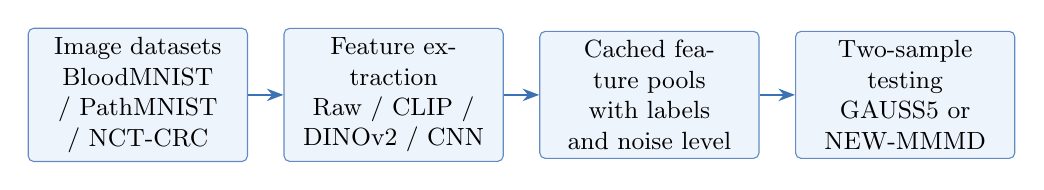
\begin{tikzpicture}[
  node distance=0.45cm,
  flowbox/.style={draw=fudanblue!65, fill=fudanlight, rounded corners=2pt,
                  minimum height=0.78cm, text width=2.55cm, align=center, font=\small},
  arr/.style={-{Stealth[length=2.1mm]}, thick, draw=fudanblue!80}
]
  \node[flowbox] (data) {Image datasets\\BloodMNIST / PathMNIST / NCT-CRC};
  \node[flowbox, right=of data] (repr) {Feature extraction\\Raw / CLIP / DINOv2 / CNN};
  \node[flowbox, right=of repr] (pool) {Cached feature pools\\with labels and noise level};
  \node[flowbox, right=of pool] (test) {Two-sample testing\\GAUSS5 or NEW-MMMD};
  \draw[arr] (data) -- (repr);
  \draw[arr] (repr) -- (pool);
  \draw[arr] (pool) -- (test);
\end{tikzpicture}
\end{center}

\vspace{0.18cm}
\scriptsize
\begin{tabularx}{0.96\linewidth}{lXX}
\toprule
Study & Main comparison & Main question \\
\midrule
BloodMNIST noise & Raw / CLIP / DINOv2 / CNN across six noise levels & Which representation is robust to image noise? \\
BloodMNIST sample size & Raw / CLIP / DINOv2 at $\sigma=0.6$ & How many samples are needed for useful power? \\
PathMNIST alignment & CLIP / DINOv2 versus trained CNN baselines & Do frozen encoders match the reproduction CNN? \\
NCT-CRC testing layer & GEXP-5 versus NEW-MMMD across representations & Does stabilization improve power or calibration? \\
\bottomrule
\end{tabularx}
\vspace{0.12cm}
\begin{center}
\smallnote{This organization avoids mixing three different factors: dataset difficulty, representation quality, and testing-layer stabilization.}
\end{center}
\end{frame}

% -------------------------------------------------------------------
\begin{frame}{BloodMNIST-224 Noise Study}{Task-trained CNN is most robust under image noise}
\begin{columns}[T,totalwidth=\linewidth]
\begin{column}{0.61\linewidth}
  \fig[width=\linewidth,height=0.56\textheight,keepaspectratio]{foundation_bloodmnist_representation_comparison.png}
\end{column}
\begin{column}{0.35\linewidth}
  \scriptsize
  \textbf{Question:} which representation survives additive image noise?

  \vspace{0.20em}
  \textbf{Task:} balanced mixtures $(0,1,3)$ vs $(0,1,6)$.

  \vspace{0.35em}
  \begin{tabular}{lcc}
  \toprule
  Method & $\sigma=0$ & $\sigma=1$ \\
  \midrule
  Raw & 0.676 & 0.515 \\
  CLIP & 0.980 & 0.315 \\
  DINOv2 & 0.922 & 0.429 \\
  CNN final & \textbf{0.993} & \textbf{0.917} \\
  \bottomrule
  \end{tabular}

  \vspace{0.40em}
  \begin{itemize}
    \item CLIP and DINOv2 are strong at low-to-medium noise.
    \item CNN final features retain high power even at heavy noise.
    \item Matched-null Type-I error stays close to nominal after correcting the fixed-pool null design.
  \end{itemize}
\end{column}
\end{columns}
\end{frame}

% -------------------------------------------------------------------
\begin{frame}{PathMNIST-28 Alignment Study}{DINOv2 catches up with larger sample size}
\begin{columns}[T,totalwidth=\linewidth]
\begin{column}{0.58\linewidth}
  \fig[width=\linewidth,height=0.51\textheight,keepaspectratio]{foundation_pathmnist_vs_cnn.png}
\end{column}
\begin{column}{0.38\linewidth}
  \scriptsize
  \textbf{Question:} can frozen encoders match the trained-CNN reproduction baseline?

  \vspace{0.20em}
  \textbf{Task:} reproduction-aligned overlapping-mixture setting.

  \vspace{0.30em}
  \begin{tabular}{ccc}
  \toprule
  $n$ & CLIP & DINOv2 \\
  \midrule
  30 & 0.117 & 0.053 \\
  60 & 0.176 & 0.251 \\
  90 & 0.323 & 0.593 \\
  120 & 0.515 & 0.890 \\
  150 & 0.717 & 0.990 \\
  \bottomrule
  \end{tabular}

  \vspace{0.25em}
  \begin{itemize}
    \item DINOv2 is much stronger than CLIP once sample size grows.
    \item Small images still favor task-trained CNNs in the small-to-medium sample regime.
  \end{itemize}
\end{column}
\end{columns}
\end{frame}

% -------------------------------------------------------------------
\begin{frame}{NCT-CRC Representation Study}{DINOv2 overtakes CNN at larger sample sizes}
\begin{columns}[T,totalwidth=\linewidth]
\begin{column}{0.61\linewidth}
  \fig[width=\linewidth,height=0.56\textheight,keepaspectratio]{foundation_nctcrc_representation_comparison.png}
\end{column}
\begin{column}{0.35\linewidth}
  \scriptsize
  \textbf{Question:} how do representations scale with sample size on larger pathology images?

  \vspace{0.20em}
  \textbf{Task:} $(\mathrm{NORM,STR,LYM})$ vs $(\mathrm{TUM,STR,LYM})$.

  \vspace{0.35em}
  \begin{tabular}{ccccc}
  \toprule
  $n$ & Raw & CLIP & CNN & DINO \\
  \midrule
  30 & .125 & .013 & .100 & .038 \\
  60 & .113 & .063 & .288 & .188 \\
  90 & .175 & .200 & .575 & .475 \\
  120 & .238 & .500 & .738 & .875 \\
  150 & .300 & .750 & .875 & \textbf{.988} \\
  \bottomrule
  \end{tabular}

  \vspace{0.40em}
  \begin{itemize}
    \item CNN is stronger at small-to-medium sample sizes.
    \item DINOv2 becomes best when sample size reaches 120--150.
    \item Raw pixels remain sample-inefficient.
  \end{itemize}
\end{column}
\end{columns}
\end{frame}

% -------------------------------------------------------------------
\begin{frame}{NEW-MMMD Testing-Layer Study}{Stabilization helps calibration more than it guarantees power}
\begin{columns}[T,totalwidth=\linewidth]
\begin{column}{0.63\linewidth}
  \fig[width=\linewidth,height=0.48\textheight,keepaspectratio]{foundation_nctcrc_newmmmd_comparison.png}
\end{column}
\begin{column}{0.33\linewidth}
  \scriptsize
  \textbf{Question:} after fixing the representation, does the stabilized test improve the final decision?

  \vspace{0.20em}
  \textbf{Comparison:} GEXP-5 versus NEW-MMMD on NCT-CRC.

  \vspace{0.25em}
  \begin{itemize}
    \item NEW-MMMD uses covariance stabilization and kernel pruning.
    \item It often lowers Type-I error and improves conditioning.
    \item It does not uniformly increase power; small samples can lose power.
    \item At large $n$, it can match GEXP-5 for DINOv2 and CNN.
  \end{itemize}
\end{column}
\end{columns}
\end{frame}

% -------------------------------------------------------------------
\begin{frame}{Takeaways from Foundation-Encoder Experiments}{Interpreting the empirical patterns}
\keyline{Two-sample testing is strongly shaped by the geometry of the representation space.}
\vspace{0.08cm}
\scriptsize
\begin{tabularx}{0.96\linewidth}{>{\bfseries\color{fudanblue}}p{0.27\linewidth}X}
\toprule
Observation & Interpretation \\
\midrule
Raw pixels are weakest
& No invariance; high-dimensional distances are noisy and dominated by nuisance variation. \\
\addlinespace[0.18em]
CNN is strongest on BloodMNIST
& Task-trained cell morphology features; convolution and pooling filter pixel-level noise. \\
\addlinespace[0.18em]
DINOv2 wins on large NCT-CRC samples
& Pretrained visual features capture richer tissue architecture; advantage appears at larger $n$. \\
\addlinespace[0.18em]
DINOv2 $>$ CLIP
& Morphology and texture matter more than language-level semantics. \\
\addlinespace[0.18em]
NEW-MMMD is conservative
& Better calibration and numerical stability; possible small-sample power tradeoff. \\
\bottomrule
\end{tabularx}

\vspace{0.20cm}
\begin{center}
\smallnote{A good embedding makes biologically meaningful differences kernel-detectable; raw pixels leave MMMD to fight high-dimensional nuisance variation directly.}
\end{center}
\end{frame}

% -------------------------------------------------------------------
\end{document}
